\section{Séance 4 : Offre de travail et de capital}


\subsection{Offre de travail}



\begin{tabular}{lll}
	Heures de travail & $\Rightarrow$ & $Tr$\\
	Heures de loisir  & $\Rightarrow$ & $Loi$\\
	Salaire horaire   & $\Rightarrow$ & $Wh$\\
	Revenu journalier & $\Rightarrow$ & $Y$\\
\end{tabular}
$$1\ journee = 24\ heures = Tr + Loi$$
$$Y = Wh * Tr$$



\subsubsection{Graphiques}



\begin{center}
	\begin{tabular}{cc}
		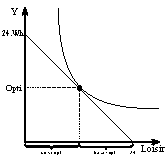
\includegraphics[width=0.25\textwidth]{images/graph_offre_de_travail.pdf} & 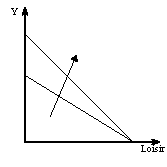
\includegraphics[width=0.25\textwidth]{images/graph_offre_de_travail_wh_augmente.pdf}\\
		Complet                                                                   & Si $Wh$ augmente
	\end{tabular}
\end{center}



\subsection{Offre de capital}



\begin{tabular}{lll}
	Consommation en 1ère période  & $\Rightarrow$ & $C_t$\\
	Consommation en 2ème période  & $\Rightarrow$ & $C_{t+1}$\\
	Revenu en 1ère période        & $\Rightarrow$ & $Y_t$\\
	Revenu en 2ee période         & $\Rightarrow$ & $Y_{t+2}$\\
	Épargne                       & $\Rightarrow$ & $S_t$\\
	Taux d'intérêt                & $\Rightarrow$ & $r$\\
	Cherche à maximiser l'utilité & $\Rightarrow$ & $U(C_t,C_{t+1})$
\end{tabular}
$$S_t = Y_t - C_t$$
\begin{flushright}
	(si St < 0 : emprunt)
\end{flushright}
$$C_{t+1} = Y_{t+1} + ( 1 + r ) * S_t $$



\subsubsection{Graphiques}



\begin{center}
	\begin{tabular}{ccc}
		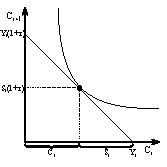
\includegraphics[width=0.25\textwidth]{images/graph_offre_de_capital.pdf} & 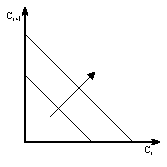
\includegraphics[width=0.25\textwidth]{images/graph_offre_de_capital_y_t_augmente.pdf} & 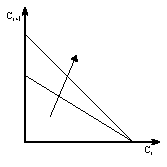
\includegraphics[width=0.25\textwidth]{images/graph_offre_de_capital_r_augmente.pdf}\\
		Complet             &             Si $Y_t$ augmente             &             Si $r$ augmente
	\end{tabular}
\end{center}